\begin{tikzpicture}
\tikzstyle{eng-step} = [draw, thick, fill=white, align=center, minimum width=1cm, minimum height=1cm]


%%% Switch %%%

\coordinate (s) at (-1.0, 0);
\node[eng-step, rotate=270] (switch)  at (0, 0) {\Large \faSitemap};

%%% Controllers %%%

\node[eng-step] (c2) at (-2.25, 0.15) {\Large$\mathcal{C}$};
\node[eng-step] (c1) at (-2.10, 0) {\Large$\mathcal{C}$};
\coordinate (c) at (-4, 0);

%%%% Plant %%%

\node[eng-step] (plant)     at (2.5,0) {\Large$\mathcal{P}$};
\coordinate (p2) at (4, -2);

%%%%%%%%%%%%%%%
%%%% ARROWS %%%
%%%%%%%%%%%%%%%

\draw[-latex,thick] (c1.east) to (switch.south);

\draw[-latex,thick] (switch.north) to (plant.west);

\draw[-,thick] (plant.east)  -| (p2) -| (c);

\draw[-latex,thick] (c) to (c1.west);

\end{tikzpicture}
